%\textsl{}%!TEX TS-options = --shell-escape
%!TEX TS-program = pdflatex
\documentclass[%
   10pt,              % Schriftgroesse
   ngerman,           % wird an andere Pakete weitergereicht
   a4paper,           % Seitengroesse
   DIV11,             % Textbereichsgroesse (siehe Koma Skript Dokumentation !)
]{scrartcl}%     Klassen: scrartcl, scrreprt, scrbook, article
% -------------------------------------------------------------------------

\usepackage[utf8]{inputenc} % Font Encoding, benoetigt fuer Umlaute
\usepackage[english]{babel}   % \textsl{}Spracheinstellung

\usepackage[T1]{fontenc} % T1 Schrift Encoding
\usepackage{textcomp}    % Zusatzliche Symbole (Text Companion font extension)
\usepackage{lmodern,dsfont}     % Latin Modern Schrift
\usepackage{dsfont}
%\usepackage{wasysym}
\usepackage{ulem}
\usepackage{graphicx}
\usepackage{eurosym}
%\usepackage{txfonts}
\usepackage{stmaryrd}
\usepackage{amsfonts}
\usepackage{amsmath}
\usepackage{hyperref}
\usepackage{tikz}
\usepackage{multirow}
\usepackage{listings}
\usepackage{etextools}
\usepackage{ifthen}
%\usepackage{TikZ} %phylogenetischer Baum
%\usetikzlibrary{calc, shapes, backgrounds} %für die Phylogenetische bäume
%\usetikzlibrary{automata,arrows}
\usepackage{subfigure} 


% Definition des Headers
\usepackage{geometry}
\geometry{a4paper, top=3cm, left=3cm, right=3cm, bottom=3cm, headsep=0mm, footskip=0mm}
\renewcommand{\baselinestretch}{1.3}\normalsize

\def\header#1#2#3#4#5#6#7{\pagestyle{empty}
\noindent
\begin{minipage}[t]{0.6\textwidth}
\begin{flushleft}
\textbf{#4}\\% Fach
#6\\% Semester
Tutor: #2  % Tutor 
\end{flushleft}
\end{minipage}
\begin{minipage}[t]{0.4\textwidth}
\begin{flushright}
\points{#7}% Punktetabelle
\vspace*{0.2cm}
#5%  Names
\end{flushright}
\end{minipage}

\begin{center}
{\Large\textbf{ Blatt #1}} % Blatt

{(Abgabe am #3)} % Abgabedatum
\end{center}
}

\newenvironment{vartab}[1]
{
    \begin{tabular}{ |c@{} *{#1}{c|} } %\hline
}{
    \end{tabular}
}

\newcommand{\myformat}[1]{& #1}

\newcommand{\entry}[1]{
  \edef\result{\csvloop[\myformat]{#1}}
  \result \\ \hline
}

\newcommand{\numbers}[1]{
  \newcounter{ctra}
\setcounter{ctra}{1}
\whiledo {\value{ctra} < #1}%
{%
  \myformat{\thectra}
  \stepcounter{ctra}%
}
\myformat{\thectra}
}
\newcommand{\emptyLine}[1]{
  \newcounter{ctra1}
\setcounter{ctra}{1}
\whiledo {\value{ctra1} < #1}%
{%
  \myformat{\hspace*{0.5cm}}
  \stepcounter{ctra1}%
}
}

\newcommand{\points}[1]{
\newcounter{colmns}
\setcounter{colmns}{#1}
\stepcounter{colmns}
  \begin{vartab}{\thecolmns}
    \numbers{#1} & $\sum$ (6+2)\\\hline
    \emptyLine{\thecolmns}\\
  \end{vartab}
}

\begin{document}
%\header{Blatt}{Tutor}{Abgabedatum}{Vorlesung}{Bearbeiter}{Semester}{Anzahl Aufgaben}
\header{9}{Alexander Seitz}{18. January 2016}{Bioinformatics I}{\\Jonas Ditz \\\& Benjamin Schroeder}{WS 15/16}{4}

\section*{Theoretical Assignment - \textit{Overlap and Layout}}
\subsection*{graphs}
The graphs from the exercise are shown in Figure 1-2. Figure \ref{fig:og} is the overlap grap with minimal spanning tree (red edges) and Figure \ref{fig:layout} shows the layout. 
	 
\begin{figure}[h]
	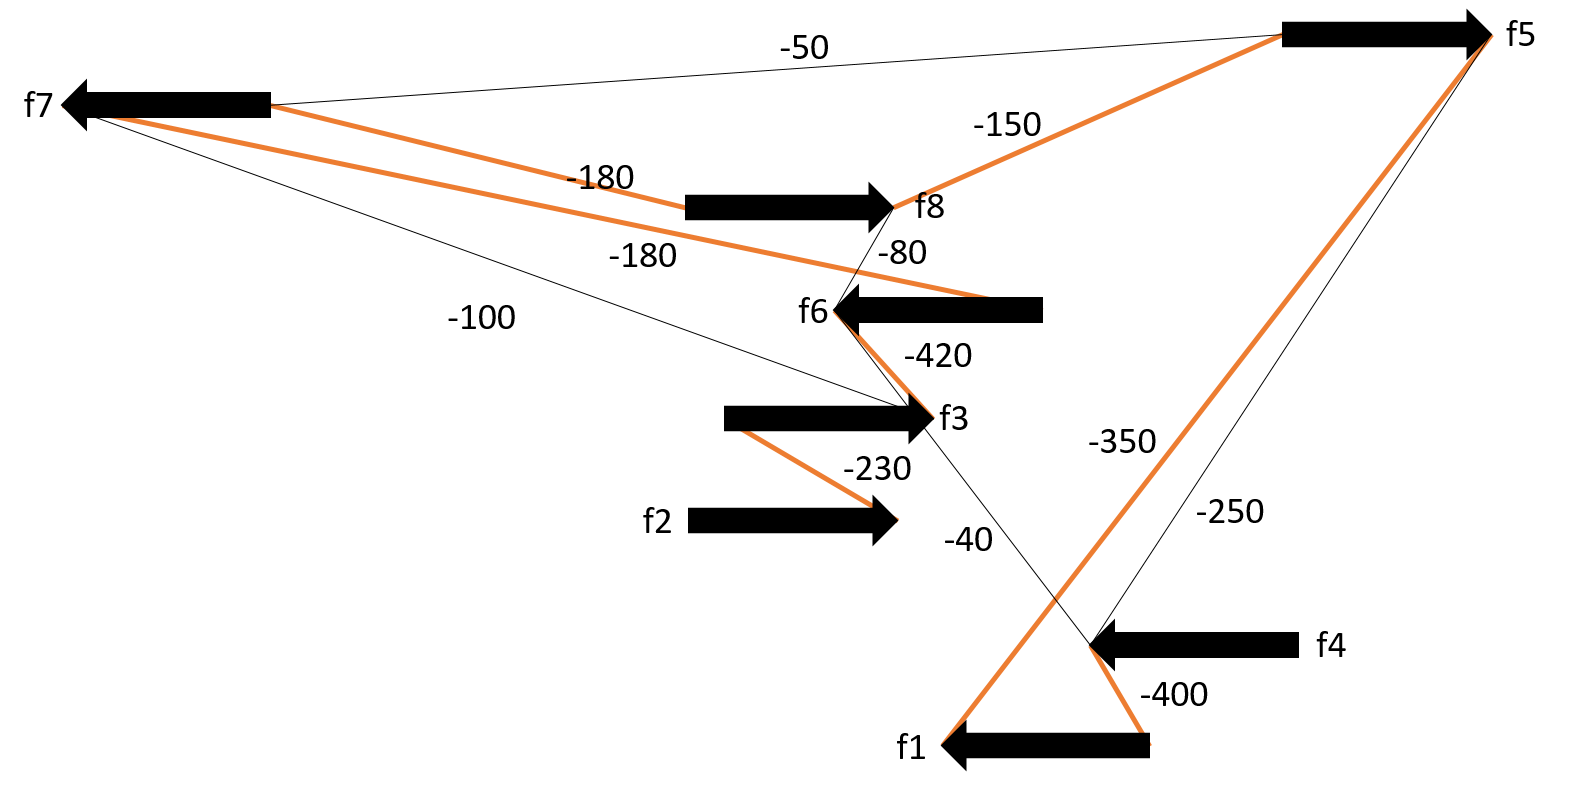
\includegraphics[width=\textwidth]{minimal-Spanning-Tree.png}
	\caption{Minimal-spanning-tree}
	\label{fig:og}
\end{figure}


\begin{figure}[h]
	
\includegraphics[width=\textwidth]{layout.png}
	\caption{layout}
	\label{fig:layout}
\end{figure}

\subsection*{Is the Layout consitent?}
One overlap ($f_6$ and $f_8$) is not consistent, because:
\begin{equation*}
o(3'f_6 - 3'f_8)=80
\end{equation*}
\section*{Theoretical Assignment - \textit{Overlap graph figure}}
 
A Figure for a paper would look like Figure \ref{fig:paper}.

\begin{figure}[h]
	\centering
	\subfigure{
		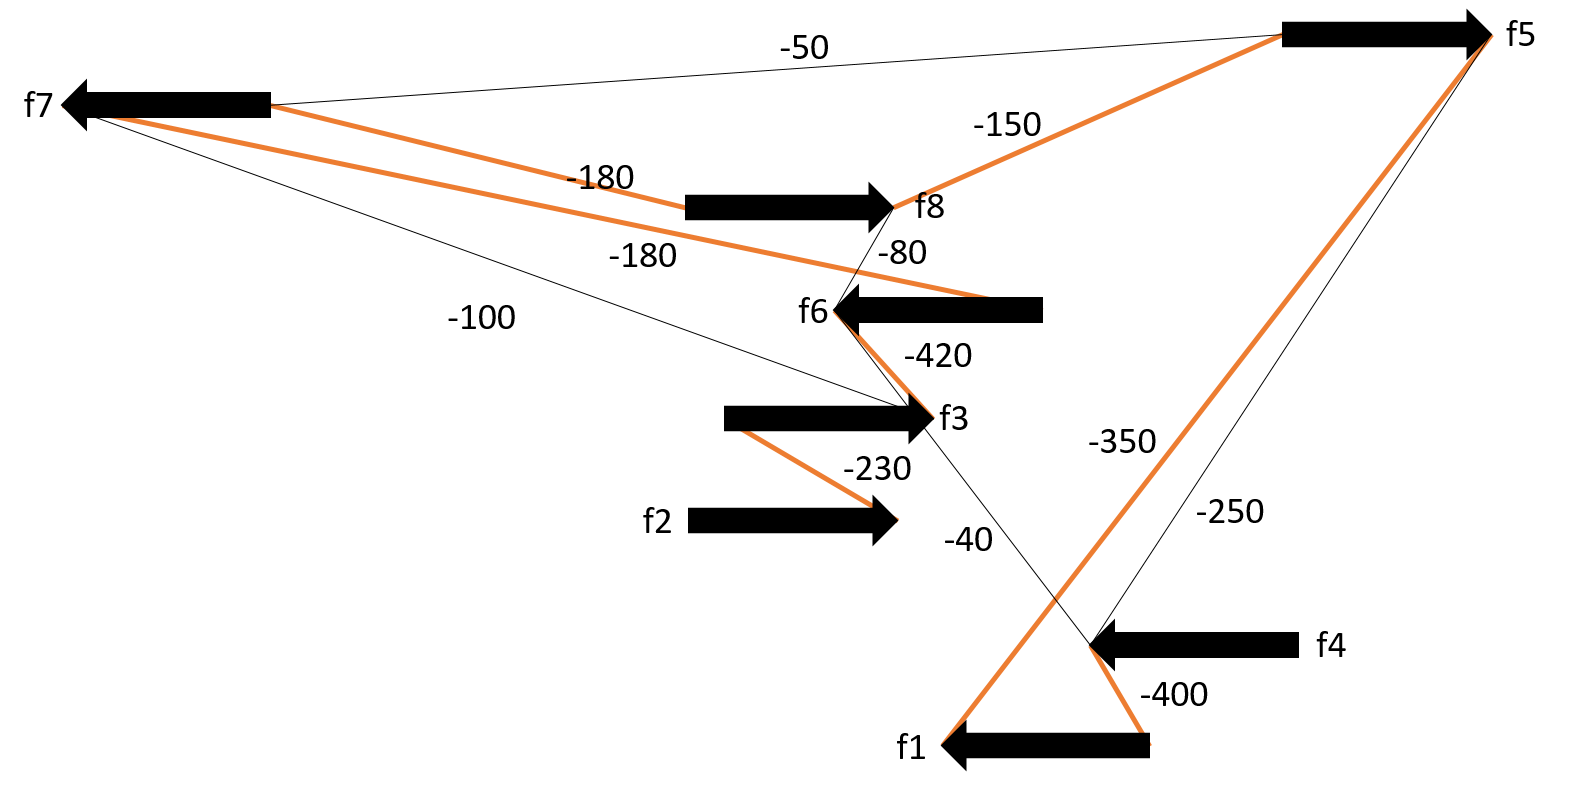
\includegraphics[width=0.45\textwidth]{minimal-Spanning-Tree.png}
	}
	\subfigure{
		
\includegraphics[width=0.45\textwidth]{layout.png}
	}
	\caption{\textbf{left}: Overlap Graph with minimal spanning tree in red. \textbf{right}: Layout computed with the minimal spanning tree shown on the left site.}
	\label{fig:paper}
\end{figure} 
 
\section*{Theoretical Assignment - \textit{Computing all overlaps using suffix tree}}

Finding all overlaps is basically a APSP (All-pairs-suffix-prefix) problem. Solving such a problem 
with a suffix tree approach has a time complexity of $O(n + k^2)$ where $n$ is the total length of 
all strings and $k$ is the count of strings. First all reads will be concatenated with a separation 
character between all reads and a terminal character at the end. Now it is rather simple to check, 
whether the prefix of one read matches with the suffix of another read. This can be done using the 
suffix tree since we know that each prefix starts with an separation character (one could put one 
separation character at the beginning of the string to make this statement true) and every suffix 
ends ether with the separation character or the terminal character. Since one has to go trough the 
whole concatenated string and compare the prefix of each read with the suffix of every other read, 
this approach has a total runtime complexity of $O(n+k^2)$.

\section*{Bonus - \textit{Challenges of your Project}}

One of the biggest challenges during our project was the framework we chose, Vaadin. We were not able 
to get it working of all computers we used. So in the end it was just one of us, who was able to work 
on the front-end layer. That slowed us down a lot. If we would start this project again from the scratch, 
Django would be a better choice. This framework comes with a development server and, therefore, would 
maybe make developing together easier. In the end we wasted a lot of time with Eclipse/Vaadin/Eclipse+Vaadin 
problems. Another challenge was the database schema for POODLE. We, especially Benjamin, talked a lot 
with people from Silke Wiesner's group at the MPI for Developmental Biology and that resulted in 
several schema changes during our project time.

\end{document}